
\label{appendix:Implementation_Details}
To evaluate WAV model in real-world settings, we collected approximately 300 successful trajectories each for the drawer-opening and bowl-organization tasks, and 2,000 successful trajectories for the towel-flattening task, using a real-world Piper robot. 
Each trajectory lasts on the order of tens of seconds. Each trajectory contains RGB observations from two wrist-mounted cameras (resolution $240\times320\times3$) and one third-person top camera (resolution $240\times424\times3$), together with 14-dimensional robot joint states.
We train one task-specific model per-task and evaluate each model on the corresponding real-world scenario.
This setup enables a controlled and systematic evaluation across diverse manipulation challenges, while highlighting the robustness of the proposed WAV model in real-world deployment.

For dense reward design, we follow ReinboT~\citep{zhang2025reinbot}, which decomposes dense rewards into four aspects: sub-goal achievement, task progress, behavior smoothness, and task completion. In this work, we omit the sub-goal achievement term and retain the remaining components. Concretely, our reward consists of nine reward terms, corresponding to 16 scalar components in the bimanual setting. The definitions and weights are listed in Tab.~\ref{tab:rewards}. The dataset we use will be publicly available upon publication.

The hyperparameter configurations are summarized in Tab.~\ref{tab:trainer1} and Tab.~\ref{tab:trainer2}. Both our method and the reproduced baseline are trained using 8 NVIDIA A100-SXM4-80GB GPUs on a server equipped with Intel Xeon Platinum 8358 CPUs @ 2.60GHz. For the four LIBERO tasks, we perform full-parameter fine-tuning for 30,000 training steps on video and 40,000 training steps on value/action, which requires approximately 5 days. For the real-world Piper manipulation data, we train one model per task for 30,000 training steps on video and 30,000 training steps on value/action, which requires approximately 3 days.

\begin{table}[htbp]
\centering
\scriptsize
\setlength{\tabcolsep}{3pt}
\renewcommand{\arraystretch}{1.08}
\begin{tabularx}{\columnwidth}{p{2.9cm}Yp{2cm}}
\hline
Reward term & Definition & Weight \\
\hline
Wrist-view MSE reward
& $c_{1,t}^b=\exp\!\left(-0.01 \cdot \mathrm{MSE}(I_t^b,I_T^b)\right)$
& $+\frac{1}{16}$ each \\

Wrist-view SSIM reward
& $c_{2,t}^b=\exp\!\left(\mathrm{SSIM}(I_t^b,I_T^b)-1\right)$
& $+\frac{1}{16}$ each \\

Top-view MSE reward
& $c_{3,t}=\exp\!\left(-0.01 \cdot \mathrm{MSE}(I_t^{\mathrm{top}},I_T^{\mathrm{top}})\right)$
& $+\frac{1}{16}$ \\

Top-view SSIM reward
& $c_{4,t}=\exp\!\left(\mathrm{SSIM}(I_t^{\mathrm{top}},I_T^{\mathrm{top}})-1\right)$
& $+\frac{1}{16}$ \\

Joint-state proximity reward
& $c_{5,t}^b=\exp\!\left(-\|s_t^b-s_T^b\|_2\right)$
& $+\frac{1}{16}$ each \\

Joint velocity penalty
& $c_{6,t}^b=\sum_j |\Delta s_{t,j}^b|$
& $-\frac{1}{16}$ each \\

Joint acceleration penalty
& $c_{7,t}^b=\sum_j |\Delta^2 s_{t,j}^b|$
& $-\frac{1}{16}$ each \\

Action velocity penalty
& $c_{8,t}^b=\sum_j |\Delta a_{t,j}^b|$
& $-\frac{0.1}{16}$ each \\

Action acceleration penalty
& $c_{9,t}^b=\sum_j |\Delta^2 a_{t,j}^b|$
& $-\frac{0.1}{16}$ each \\
\hline
\end{tabularx}
\caption{Compact formulation of the dense reward terms in the bimanual setting, where $b\in\{L,R\}$ denotes the left and right arms.}
\label{tab:rewards}
\end{table}

\begin{figure}
\centering
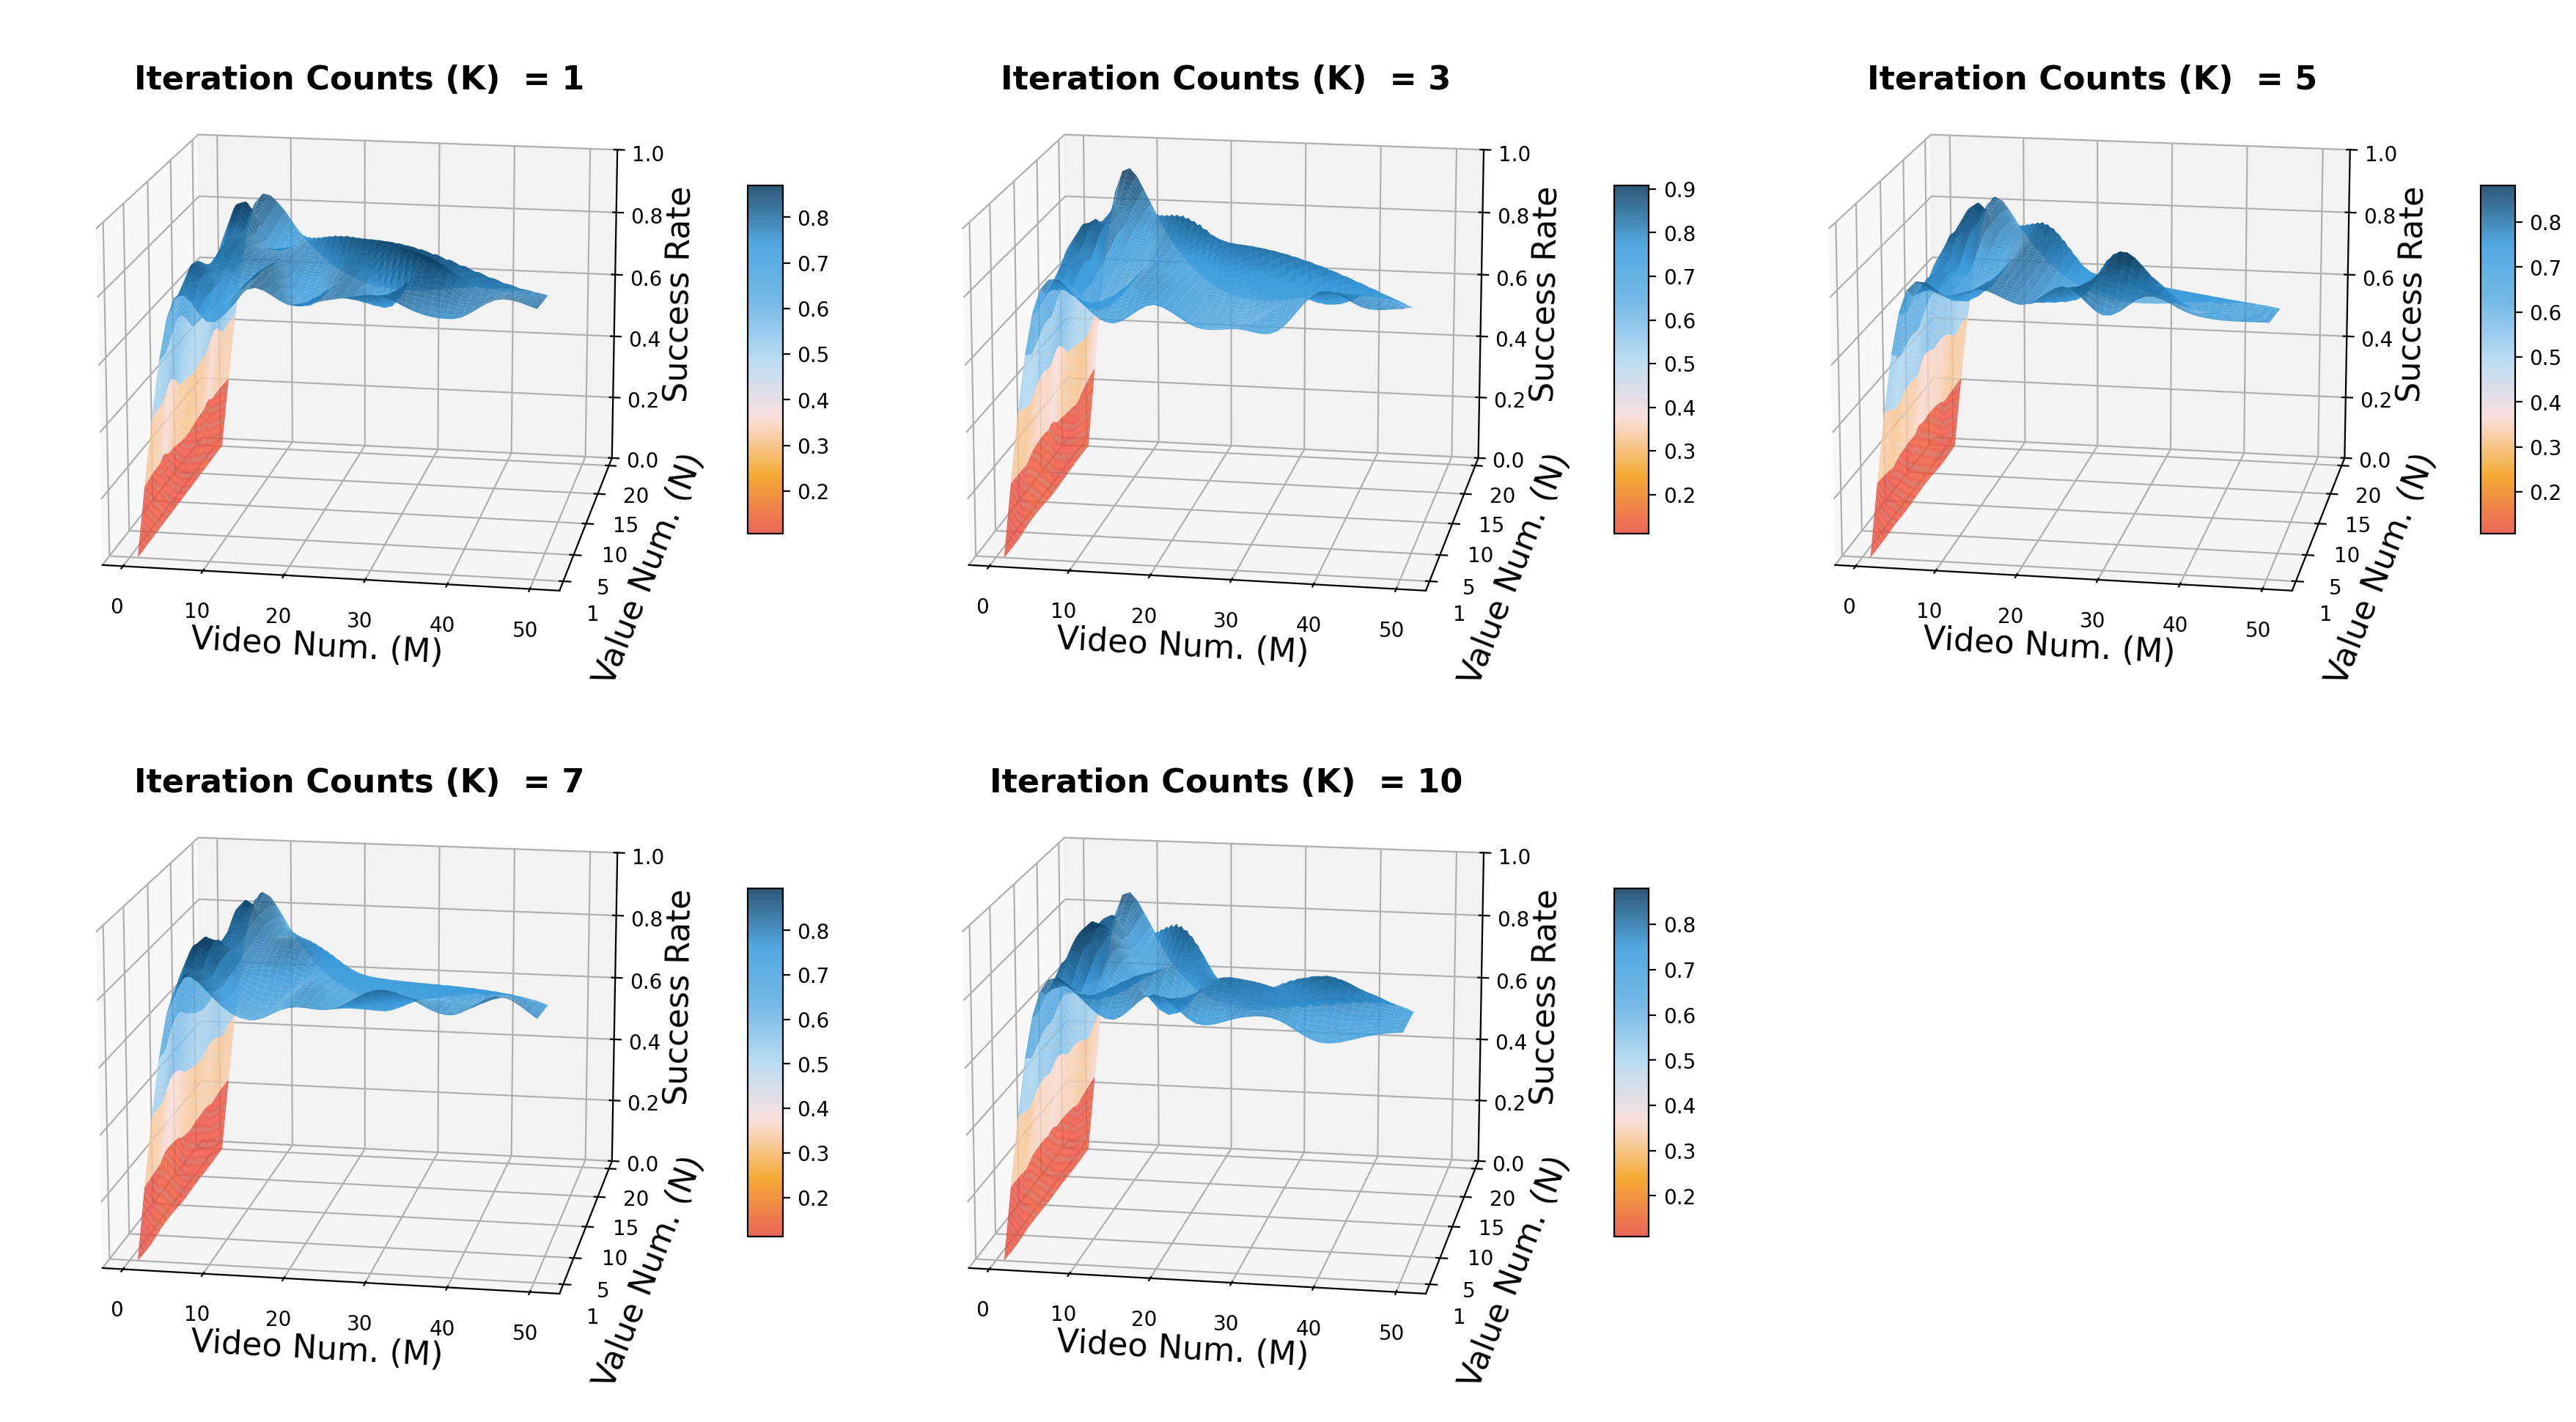
\includegraphics[width=0.95\textwidth]{figures/stage1_appendix.png}
\caption{
Performance variation trends of the WAV model under different iteration counts $K$, video latent noise sampling numbers $M$, and trajectory value noise sampling numbers $N$.
}
  \label{app_fig:stage1}
\end{figure}

\begin{figure}
\centering
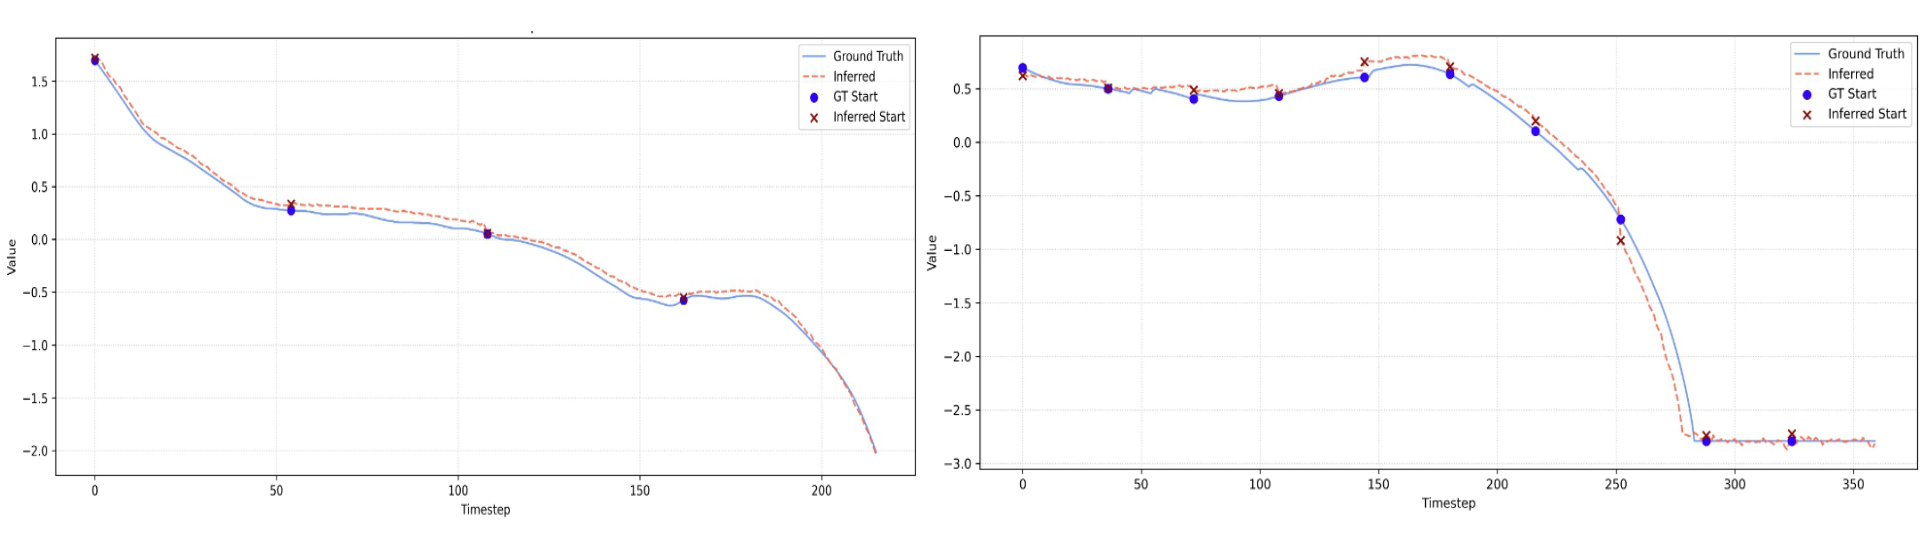
\includegraphics[width=0.95\textwidth]{figures/value.pdf}
\caption{
Comparison of inferred and ground-truth state-value trajectories in real-world robot experiments (left) and LIBERO (right).
}
  \label{app_fig:value}
\end{figure}

\begin{figure}
\centering
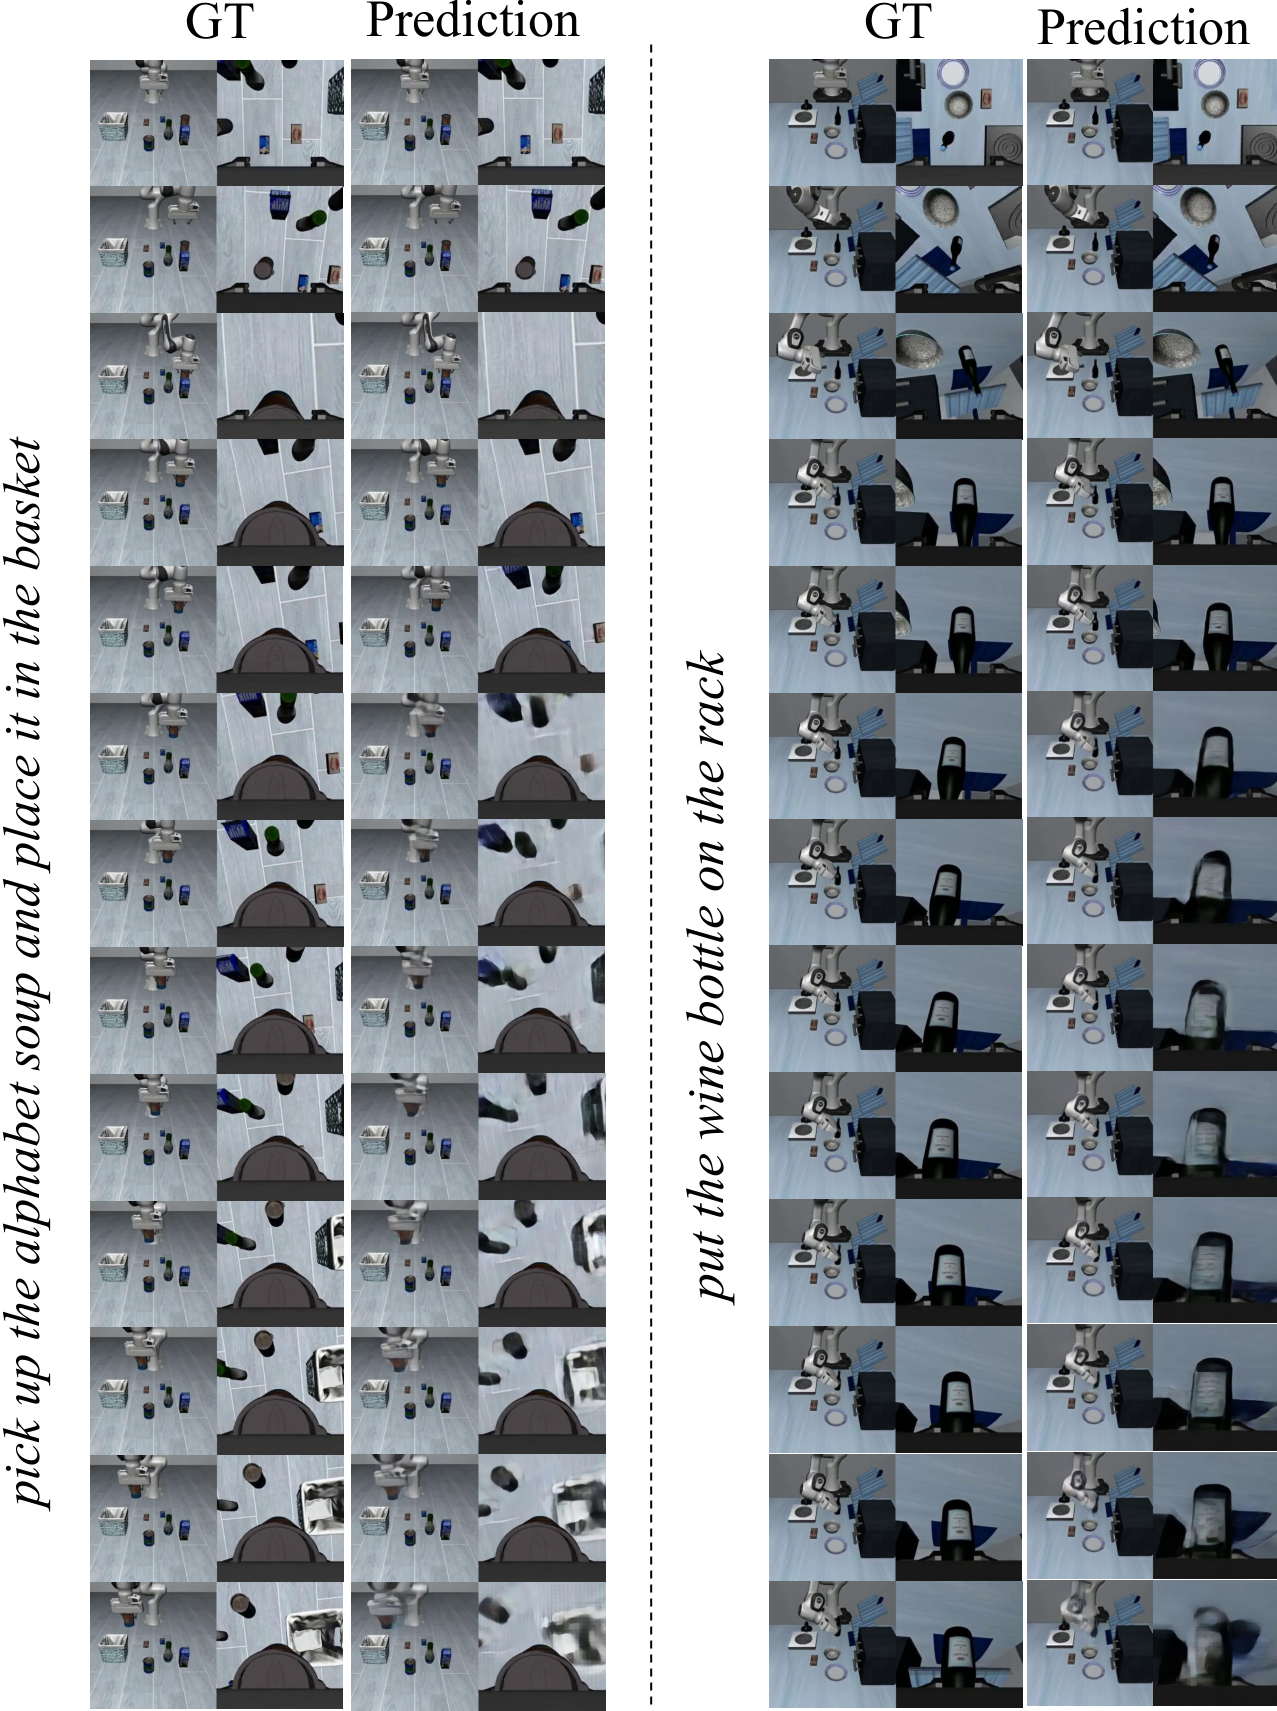
\includegraphics[width=0.95\textwidth]{figures/gt_pred_libero.pdf}
\caption{
Qualitative comparison between predicted videos and ground truth on two LIBERO tasks.
}
  \label{app_fig:gt_pred_libero}
\end{figure}

\begin{table}[htbp]
    \centering
    \caption{ Video Training hyperparameters configuration.}
        \begin{tabular}{cc}
            \toprule
            \textbf{Parameter} & \textbf{Value} \\
            \hline
            % {Training hardware} & NVIDIA A100 PCIe 80G $\times$ 8\\ 
            {Gradient clip} & 1.0 \\
            {Steps} & 40000 \\
            {Warm-up steps} & 1000 \\
            {Batch size} & 128 \\ 
            {Learning rate} & $3e-4$ \\
            {Weight decay} & $1e-5$ \\ 
            {Caption Dropout} & 0.06 \\
            {Optimizer} & Adam ($\beta_1 = 0.9, \beta_2 = 0.95, \beta_3 = 0.999$) \\ 
            \bottomrule
        \end{tabular}
    \label{tab:trainer1}
\end{table}

\begin{table}[htbp]
    \centering
    \caption{ Value \& Action Training hyperparameters configuration.}
        \begin{tabular}{cc}
            \toprule
            \textbf{Parameter} & \textbf{Value} \\
            \hline
            % {Training hardware} & NVIDIA A100 PCIe 80G $\times$ 8\\ 
            {Gradient clip} & 1.0 \\
            {Steps} & 30000 \\
            {Warm-up steps} & 1000 \\
            {Batch size} & 128 \\ 
            {Learning rate} & $5e-5$ \\
            {Weight decay} & $1e-5$ \\ 
            {Caption Dropout} & 0 \\
            {Optimizer} & Adam ($\beta_1 = 0.9, \beta_2 = 0.95, \beta_3 = 0.999$) \\ 
            \bottomrule
        \end{tabular}
    \label{tab:trainer2}
\end{table}

